\documentclass[xcolor={table}]{beamer}
\mode<presentation>{
  \usetheme{Boadilla}
  \usefonttheme[onlylarge]{structurebold}
  \usefonttheme[stillsansseriflarge]{serif}
  \setbeamerfont*{frametitle}{size=\normalsize,series=\bfseries}
  % \setbeamertemplate{navigation symbols}{}
  \setbeamercovered{transparent}
}
\usepackage[english]{babel}
\usepackage[latin1]{inputenc}
\usepackage{times}
\usepackage[T1]{fontenc}
\usepackage{amsmath}
\usepackage{amssymb}
\usepackage{esint}
\usepackage{hyperref}
\usepackage{tikz}
\usepackage{xkeyval}
\usepackage{xargs}
\usepackage{verbatim}
\usepackage{listings}
\usepackage{multimedia}
\newcommand\hmmax{0}
\newcommand\bmmax{0}
\usepackage{bm}
\usepackage{siunitx}
\usetikzlibrary{
  arrows,
  calc,
  decorations.pathmorphing,
  decorations.pathreplacing,
  decorations.markings,
  fadings,
  positioning,
  shapes,
  arrows.meta
}
\usepgfmodule{oo}

\pgfdeclareradialshading{glow2}{\pgfpoint{0cm}{0cm}}{
  color(0mm)=(white);
  color(2mm)=(white);
  color(8mm)=(black);
  color(10mm)=(black)
}
\pgfdeclareradialshading{glow}{\pgfpoint{0cm}{0cm}}{
  color(0mm)=(white);
  color(5mm)=(white);
  color(9mm)=(black);
  color(10mm)=(black)
}

\begin{tikzfadingfrompicture}[name=glow fading]
  \shade [shading=glow] (0,0) circle (1);
\end{tikzfadingfrompicture}

\begin{tikzfadingfrompicture}[name=glow2 fading]
  \shade [shading=glow2] (0,0) circle (1);
\end{tikzfadingfrompicture}

\mode<handout>{
  \usepackage{pgfpages}
  \pgfpagesuselayout{4 on 1}[a4paper,landscape,border shrink=5mm]
  \setbeamercolor{background canvas}{bg=black!10}
}

\newcommand\pgfmathsinandcos[3]{%
  \pgfmathsetmacro#1{sin(#3)}%
  \pgfmathsetmacro#2{cos(#3)}%
}
\newcommand\LongitudePlane[3][current plane]{%
  \pgfmathsinandcos\sinEl\cosEl{#2} % elevation
  \pgfmathsinandcos\sint\cost{#3} % azimuth
  \tikzset{#1/.estyle={cm={\cost,\sint*\sinEl,0,\cosEl,(0,0)}}}
}
\newcommand\LatitudePlane[3][current plane]{%
  \pgfmathsinandcos\sinEl\cosEl{#2} % elevation
  \pgfmathsinandcos\sint\cost{#3} % latitude
  \pgfmathsetmacro\yshift{\cosEl*\sint}
  \tikzset{#1/.estyle={cm={\cost,0,0,\cost*\sinEl,(0,\yshift)}}} %
}
\newcommand\DrawLongitudeCircle[2][1]{
  \LongitudePlane{\angEl}{#2}
  \tikzset{current plane/.prefix style={scale=#1}}
  % angle of "visibility"
  \pgfmathsetmacro\angVis{atan(sin(#2)*cos(\angEl)/sin(\angEl))} %
  \draw[current plane] (\angVis:1) arc (\angVis:\angVis+180:1);
  \draw[current plane,dashed] (\angVis-180:1) arc (\angVis-180:\angVis:1);
}
\newcommand\DrawLatitudeCircleArrow[2][1]{
  \LatitudePlane{\angEl}{#2}
  \tikzset{current plane/.prefix style={scale=#1}}
  \pgfmathsetmacro\sinVis{sin(#2)/cos(#2)*sin(\angEl)/cos(\angEl)}
  % angle of "visibility"
  \pgfmathsetmacro\angVis{asin(min(1,max(\sinVis,-1)))}
  \draw[current plane,decoration={markings, mark=at position 0.6 with {\arrow{<}}},postaction={decorate},line width=.6mm] (\angVis:1) arc (\angVis:-\angVis-180:1);
  \draw[current plane,dashed,line width=.6mm] (180-\angVis:1) arc (180-\angVis:\angVis:1);
}
\newcommand\DrawLatitudeCircle[2][1]{
  \LatitudePlane{\angEl}{#2}
  \tikzset{current plane/.prefix style={scale=#1}}
  \pgfmathsetmacro\sinVis{sin(#2)/cos(#2)*sin(\angEl)/cos(\angEl)}
  % angle of "visibility"
  \pgfmathsetmacro\angVis{asin(min(1,max(\sinVis,-1)))}
  \draw[current plane] (\angVis:1) arc (\angVis:-\angVis-180:1);
  \draw[current plane,dashed] (180-\angVis:1) arc (180-\angVis:\angVis:1);
}
\newcommand\coil[1]{
  {\rh * cos(\t * pi r)}, {\apart * (2 * #1 + \t) + \rv * sin(\t * pi r)}
}
\makeatletter
\define@key{DrawFromCenter}{style}[{->}]{
  \tikzset{DrawFromCenterPlane/.style={#1}}
}
\define@key{DrawFromCenter}{r}[1]{
  \def\@R{#1}
}
\define@key{DrawFromCenter}{center}[(0, 0)]{
  \def\@Center{#1}
}
\define@key{DrawFromCenter}{theta}[0]{
  \def\@Theta{#1}
}
\define@key{DrawFromCenter}{phi}[0]{
  \def\@Phi{#1}
}
\presetkeys{DrawFromCenter}{style, r, center, theta, phi}{}
\newcommand*\DrawFromCenter[1][]{
  \setkeys{DrawFromCenter}{#1}{
    \pgfmathsinandcos\sint\cost{\@Theta}
    \pgfmathsinandcos\sinp\cosp{\@Phi}
    \pgfmathsinandcos\sinA\cosA{\angEl}
    \pgfmathsetmacro\DX{\@R*\cost*\cosp}
    \pgfmathsetmacro\DY{\@R*(\cost*\sinp*\sinA+\sint*\cosA)}
    \draw[DrawFromCenterPlane] \@Center -- ++(\DX, \DY);
  }
}
\newcommand*\DrawFromCenterText[2][]{
  \setkeys{DrawFromCenter}{#1}{
    \pgfmathsinandcos\sint\cost{\@Theta}
    \pgfmathsinandcos\sinp\cosp{\@Phi}
    \pgfmathsinandcos\sinA\cosA{\angEl}
    \pgfmathsetmacro\DX{\@R*\cost*\cosp}
    \pgfmathsetmacro\DY{\@R*(\cost*\sinp*\sinA+\sint*\cosA)}
    \draw[DrawFromCenterPlane] \@Center -- ++(\DX, \DY) node {#2};
  }
}
\makeatother

% not mandatory, but I though it was better to set it blank
\setbeamertemplate{headline}{}
\def\beamer@entrycode{\vspace{-\headheight}}

\tikzstyle{snakearrow} = [decorate, decoration={pre length=0.2cm,
  post length=0.2cm, snake, amplitude=.4mm,
  segment length=2mm},thick, ->]

%% document-wide tikz options and styles

\tikzset{%
  % >=latex, % option for nice arrows
  inner sep=0pt,%
  outer sep=2pt,%
  mark coordinate/.style={inner sep=0pt,outer sep=0pt,minimum size=3pt,
    fill=black,circle}%
}
\tikzset{
  % Define standard arrow tip
  >=stealth',
  % Define style for boxes
  punkt/.style={
    rectangle,
    rounded corners,
    draw=black, very thick,
    text width=8em,
    minimum height=2.5em,
    text centered},
}

\tikzset{onslide/.code args={<#1>#2}{%
    \only<#1>{\pgfkeysalso{#2}}
    % \pgfkeysalso doesn't change the path
  }}
\tikzset{alt/.code args={<#1>#2#3}{%
    \alt<#1>{\pgfkeysalso{#2}}{\pgfkeysalso{#3}}
    % \pgfkeysalso doesn't change the path
  }}
\tikzset{temporal/.code args={<#1>#2#3#4}{%
    \temporal<#1>{\pgfkeysalso{#2}}{\pgfkeysalso{#3}}{\pgfkeysalso{#4}}
    % \pgfkeysalso doesn't change the path
  }}

\makeatletter
\newbox\@backgroundblock
\newenvironment{backgroundblock}[2]{%
  \global\setbox\@backgroundblock=\vbox\bgroup%
  \unvbox\@backgroundblock%
  \vbox to0pt\bgroup\vskip#2\hbox to0pt\bgroup\hskip#1\relax%
}{\egroup\egroup\egroup}
\addtobeamertemplate{background}{\box\@backgroundblock}{}
\makeatother

% \def\timeleft{15:00->14:55}

\title[Approximate quantum error correction]{NISQ+: Boosting quantum computing power by approximating quantum error correction}
\date{Apr. 26, 2020}
\author{Yichao Yu}
\institute{Ni Group}

\begin{document}

\begin{frame}{}
  \titlepage
\end{frame}

% A B operator (X, Z)
% Qubit state is eigen state of
\begin{frame}{Stabilizer operators}
  \begin{center}
    \begin{tikzpicture}
      \node at (0, 0) {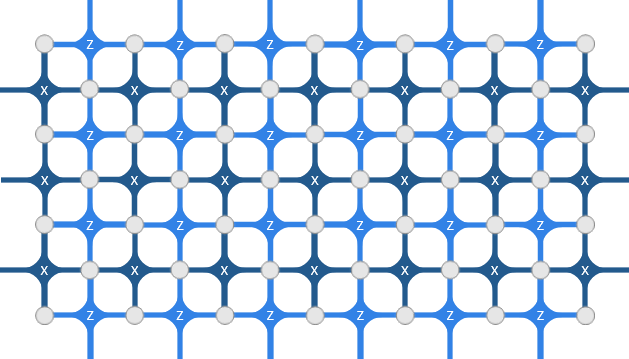
\includegraphics[width=6cm]{../2020-04-19_jc/surface_code_mesh.png}};

      \visible<2->{
        \node at (-1.8, -3) {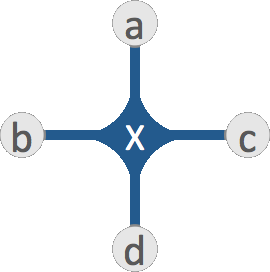
\includegraphics[width=1.6cm]{stabilizer_x.png}};
        \node[below] at (-1.8, -4) {$\displaystyle X=\prod_{i=a,b,c,d} \sigma^x_i$};

        \node at (1.8, -3) {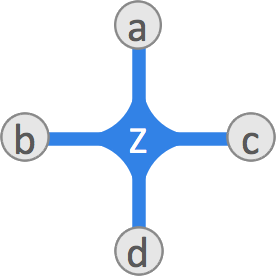
\includegraphics[width=1.6cm]{stabilizer_z.png}};
        \node[below] at (1.8, -4) {$\displaystyle Z=\prod_{i=a,b,c,d} \sigma^z_i$};
      }
    \end{tikzpicture}
  \end{center}
\end{frame}

% 1. An X or Z error happen will change the value for the (equation)
\begin{frame}{Error and stabilizer}
  \begin{center}
    \begin{tikzpicture}
      \node at (0, 0) {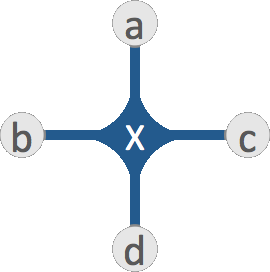
\includegraphics[width=1.6cm]{stabilizer_x.png}};
      \node[right] at (1.1, -0.2) {$\displaystyle X=\prod_{i=a,b,c,d} \sigma^x_i$};
    \end{tikzpicture}\\
    \vspace{0.6cm}
    \visible<2-> {
      Qubit state: $X|\psi\rangle=|\psi\rangle$\\
      Error: $\sigma^z_a$
    }
    \visible<3-> {
      \[X\sigma^z_a|\psi\rangle=-\sigma^z_aX|\psi\rangle=-\sigma^z_a|\psi\rangle\]
    }
  \end{center}
\end{frame}

% 2. Experimental implementation to measure X / Z eigen value
\begin{frame}{Gate implementation of stabilizer: Z}
  \begin{columns}
    \column{5cm}
    \begin{center}
      \begin{tikzpicture}
        \node at (0, 0) {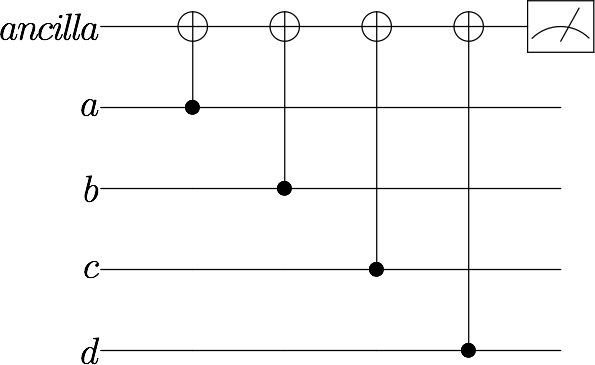
\includegraphics[width=4cm]{stabilizer_z_gate.png}};
        \node at (0, -2.5) {$\displaystyle Z=\prod_{i=a,b,c,d} \sigma^z_i$};
      \end{tikzpicture}\\
    \end{center}
    \column{6.5cm}
    \visible<2->{
      \begin{tabular}{|c|c|c|c||c|c|}
        \hline
        a&b&c&d&ancilla&$\langle Z\rangle$\\\hline
        $|0\rangle$&$|0\rangle$&$|0\rangle$&$|0\rangle$&$|0\rangle$&$1$\\\hline
        $|1\rangle$&$|0\rangle$&$|0\rangle$&$|0\rangle$&$|1\rangle$&$-1$\\\hline
        $|1\rangle$&$|1\rangle$&$|0\rangle$&$|0\rangle$&$|0\rangle$&$1$\\\hline
        $|1\rangle$&$|1\rangle$&$|1\rangle$&$|0\rangle$&$|1\rangle$&$-1$\\\hline
        $|1\rangle$&$|1\rangle$&$|1\rangle$&$|1\rangle$&$|0\rangle$&$1$\\\hline
      \end{tabular}
    }
  \end{columns}
\end{frame}

% Summary: X measure X, Z measure Z, they use the ancilla qubit but the implementation
% is not important anymore.
\begin{frame}{Gate implementation of stabilizer: X}
  \begin{center}
    \begin{tikzpicture}
      \node (Z) at (-3.2, 0) {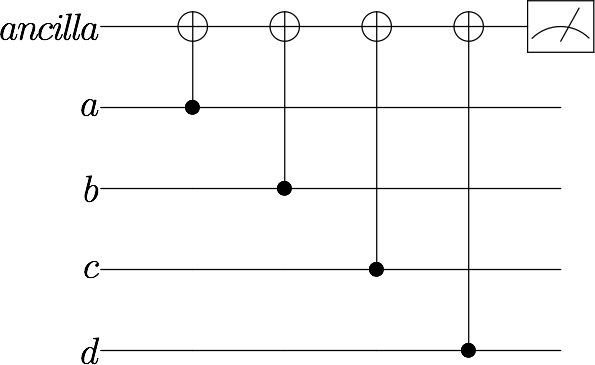
\includegraphics[height=2.2cm]{stabilizer_z_gate.png}};
      \visible<2-> {
        \node (X1) at (3.2, 0) {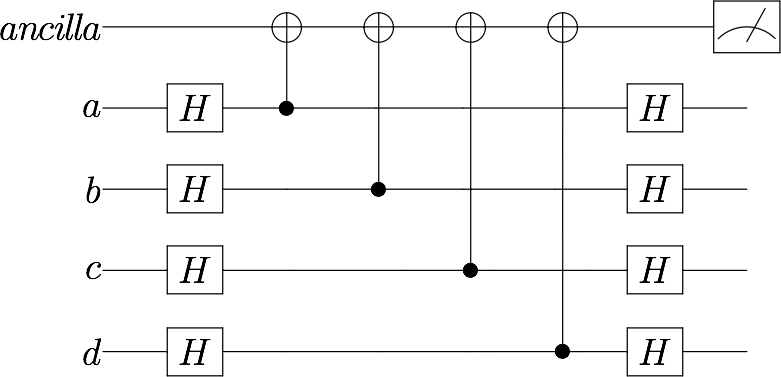
\includegraphics[height=2.2cm]{stabilizer_x_gate2.png}};
        \draw[->, blue, line width=3] (Z) -- (X1);
      }
      \visible<3-> {
        \node at (2.5, -4) {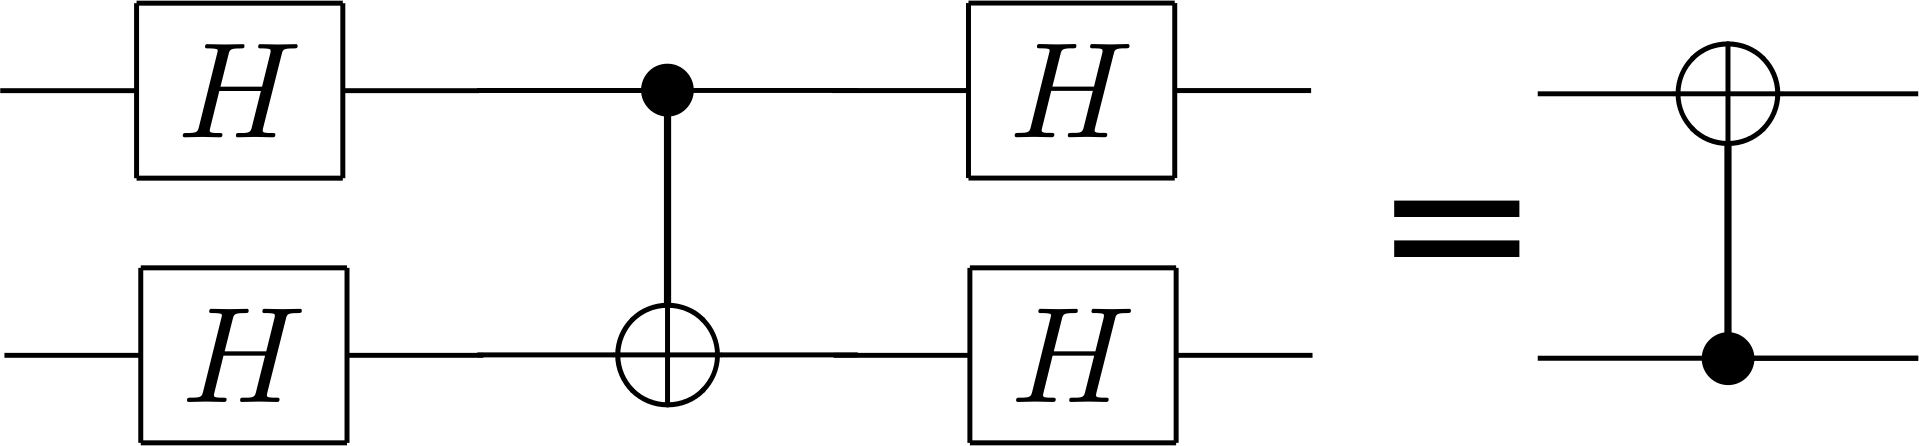
\includegraphics[width=5cm]{CNOT_Hadamard_Basis.png}};
      }
      \visible<4-> {
        \node (X2) at (-3.2, -4.5) {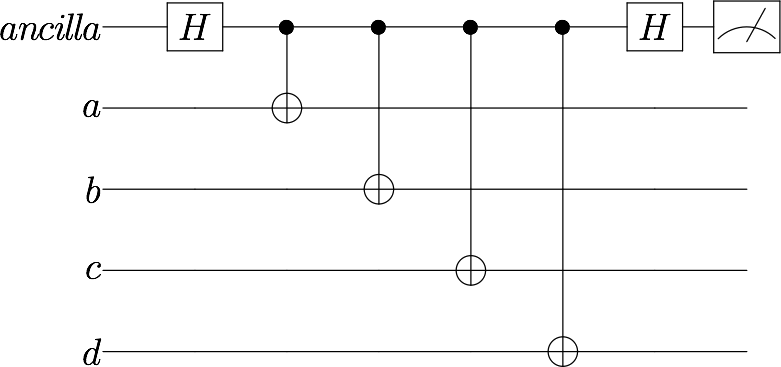
\includegraphics[height=2.2cm]{stabilizer_x_gate.png}};
        \draw[->, blue, line width=3] (X1) -- (X2);
      }
      \visible<5-> {
        \fill[white, opacity=0.92] (-5.7, -5.8) rectangle (5.7, 1.2);
      }
      \node at (-3.2, -1.8) {$\displaystyle Z=\prod_{i=a,b,c,d} \sigma^z_i$};
      \visible<2-> {
        \node at (3.2, -1.8) {$\displaystyle X=\prod_{i=a,b,c,d} \sigma^x_i$};
      }
    \end{tikzpicture}
  \end{center}
\end{frame}

\begin{frame}{Syndrome}
  \begin{center}
    \begin{tikzpicture}
      \visible<1>{
        \node at (0, 0) {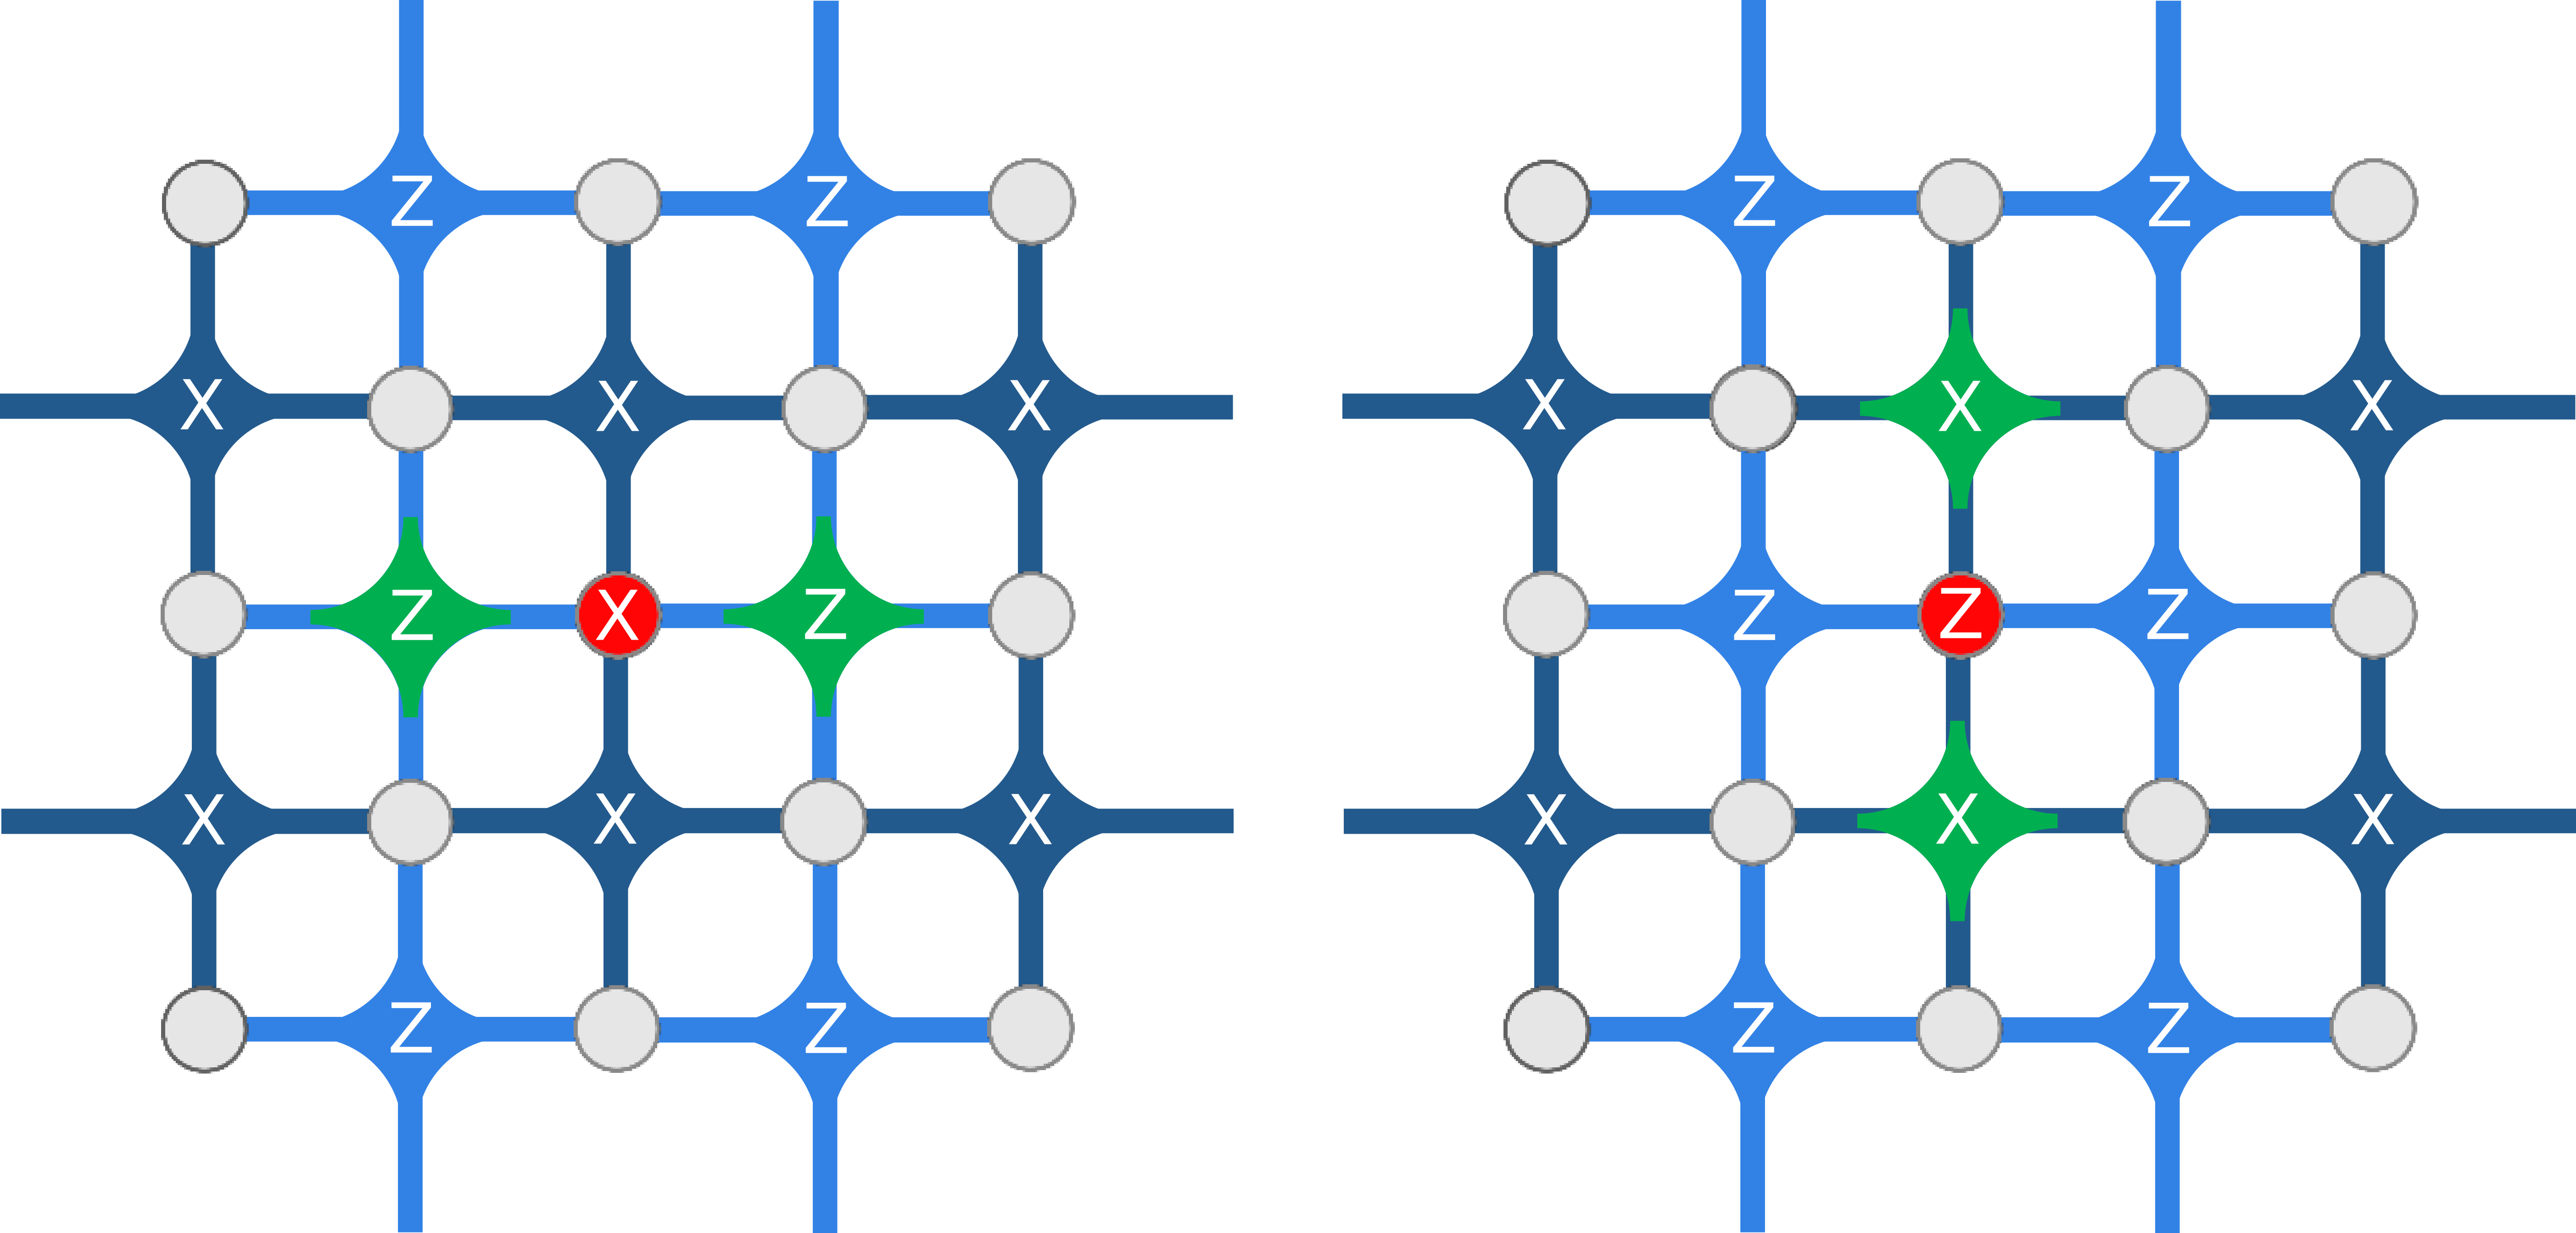
\includegraphics[height=3cm]{error_pairs.png}};
      }
      \visible<2>{
        \node at (0, 0) {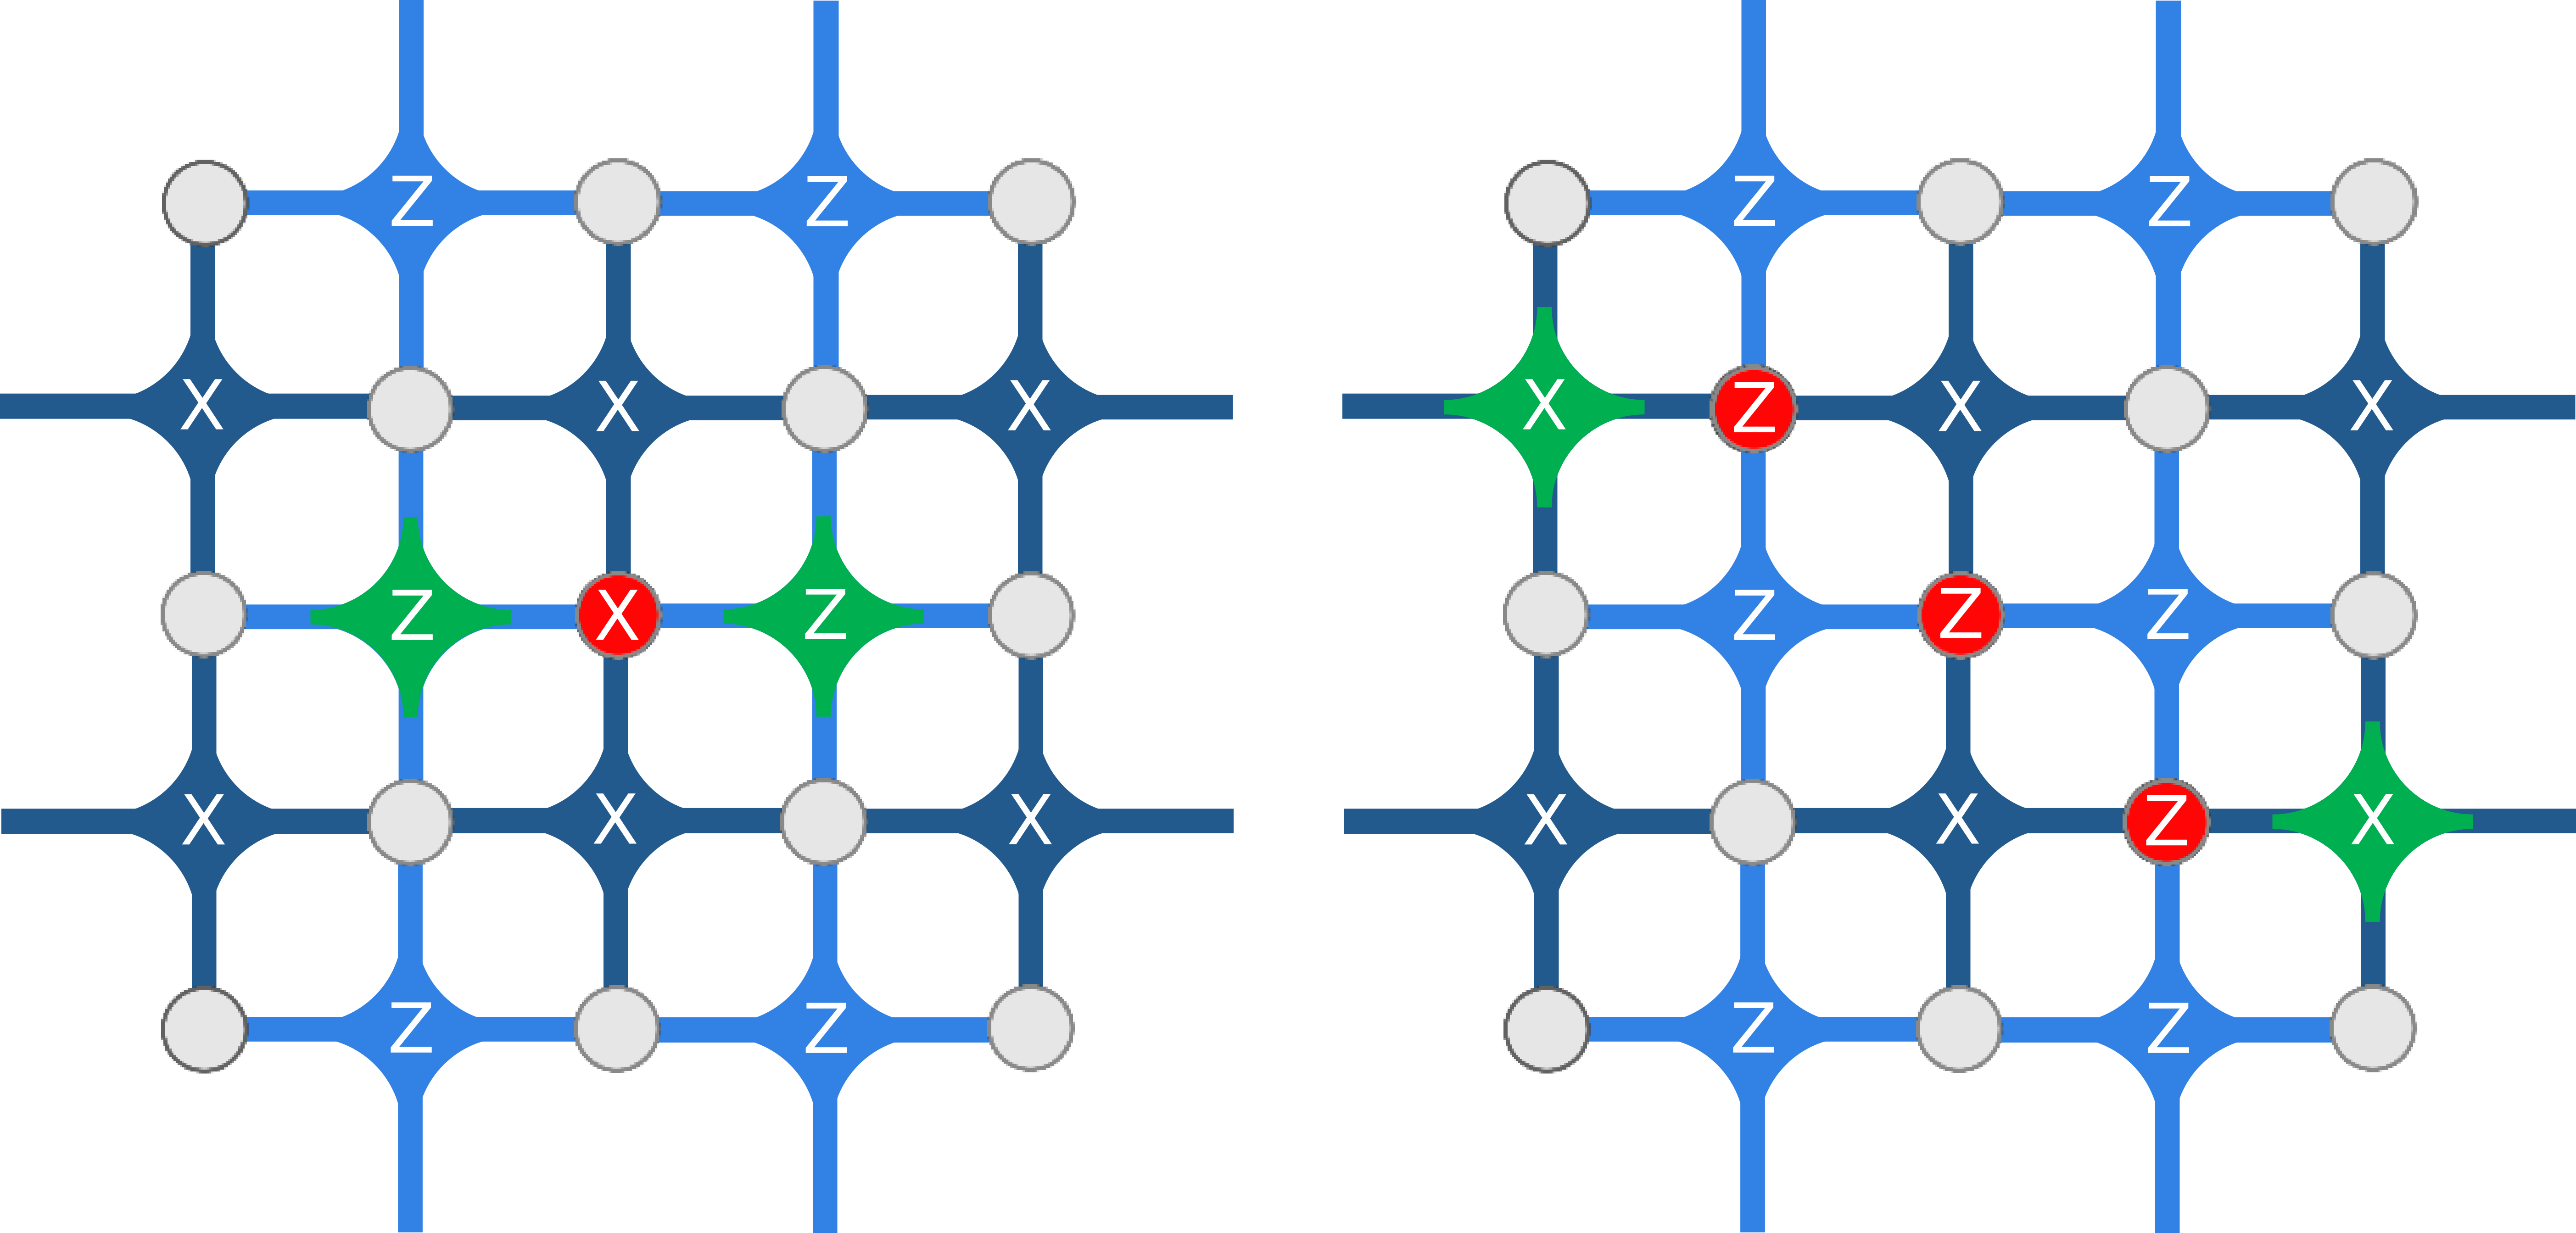
\includegraphics[height=3cm]{error_pairs2.png}};
      }
    \end{tikzpicture}
  \end{center}
\end{frame}

% Ambiguity
% String
% i.e. Loop
\begin{frame}{Benign ambiguity}
  \begin{center}
    \begin{tikzpicture}
      \node at (0, 0) {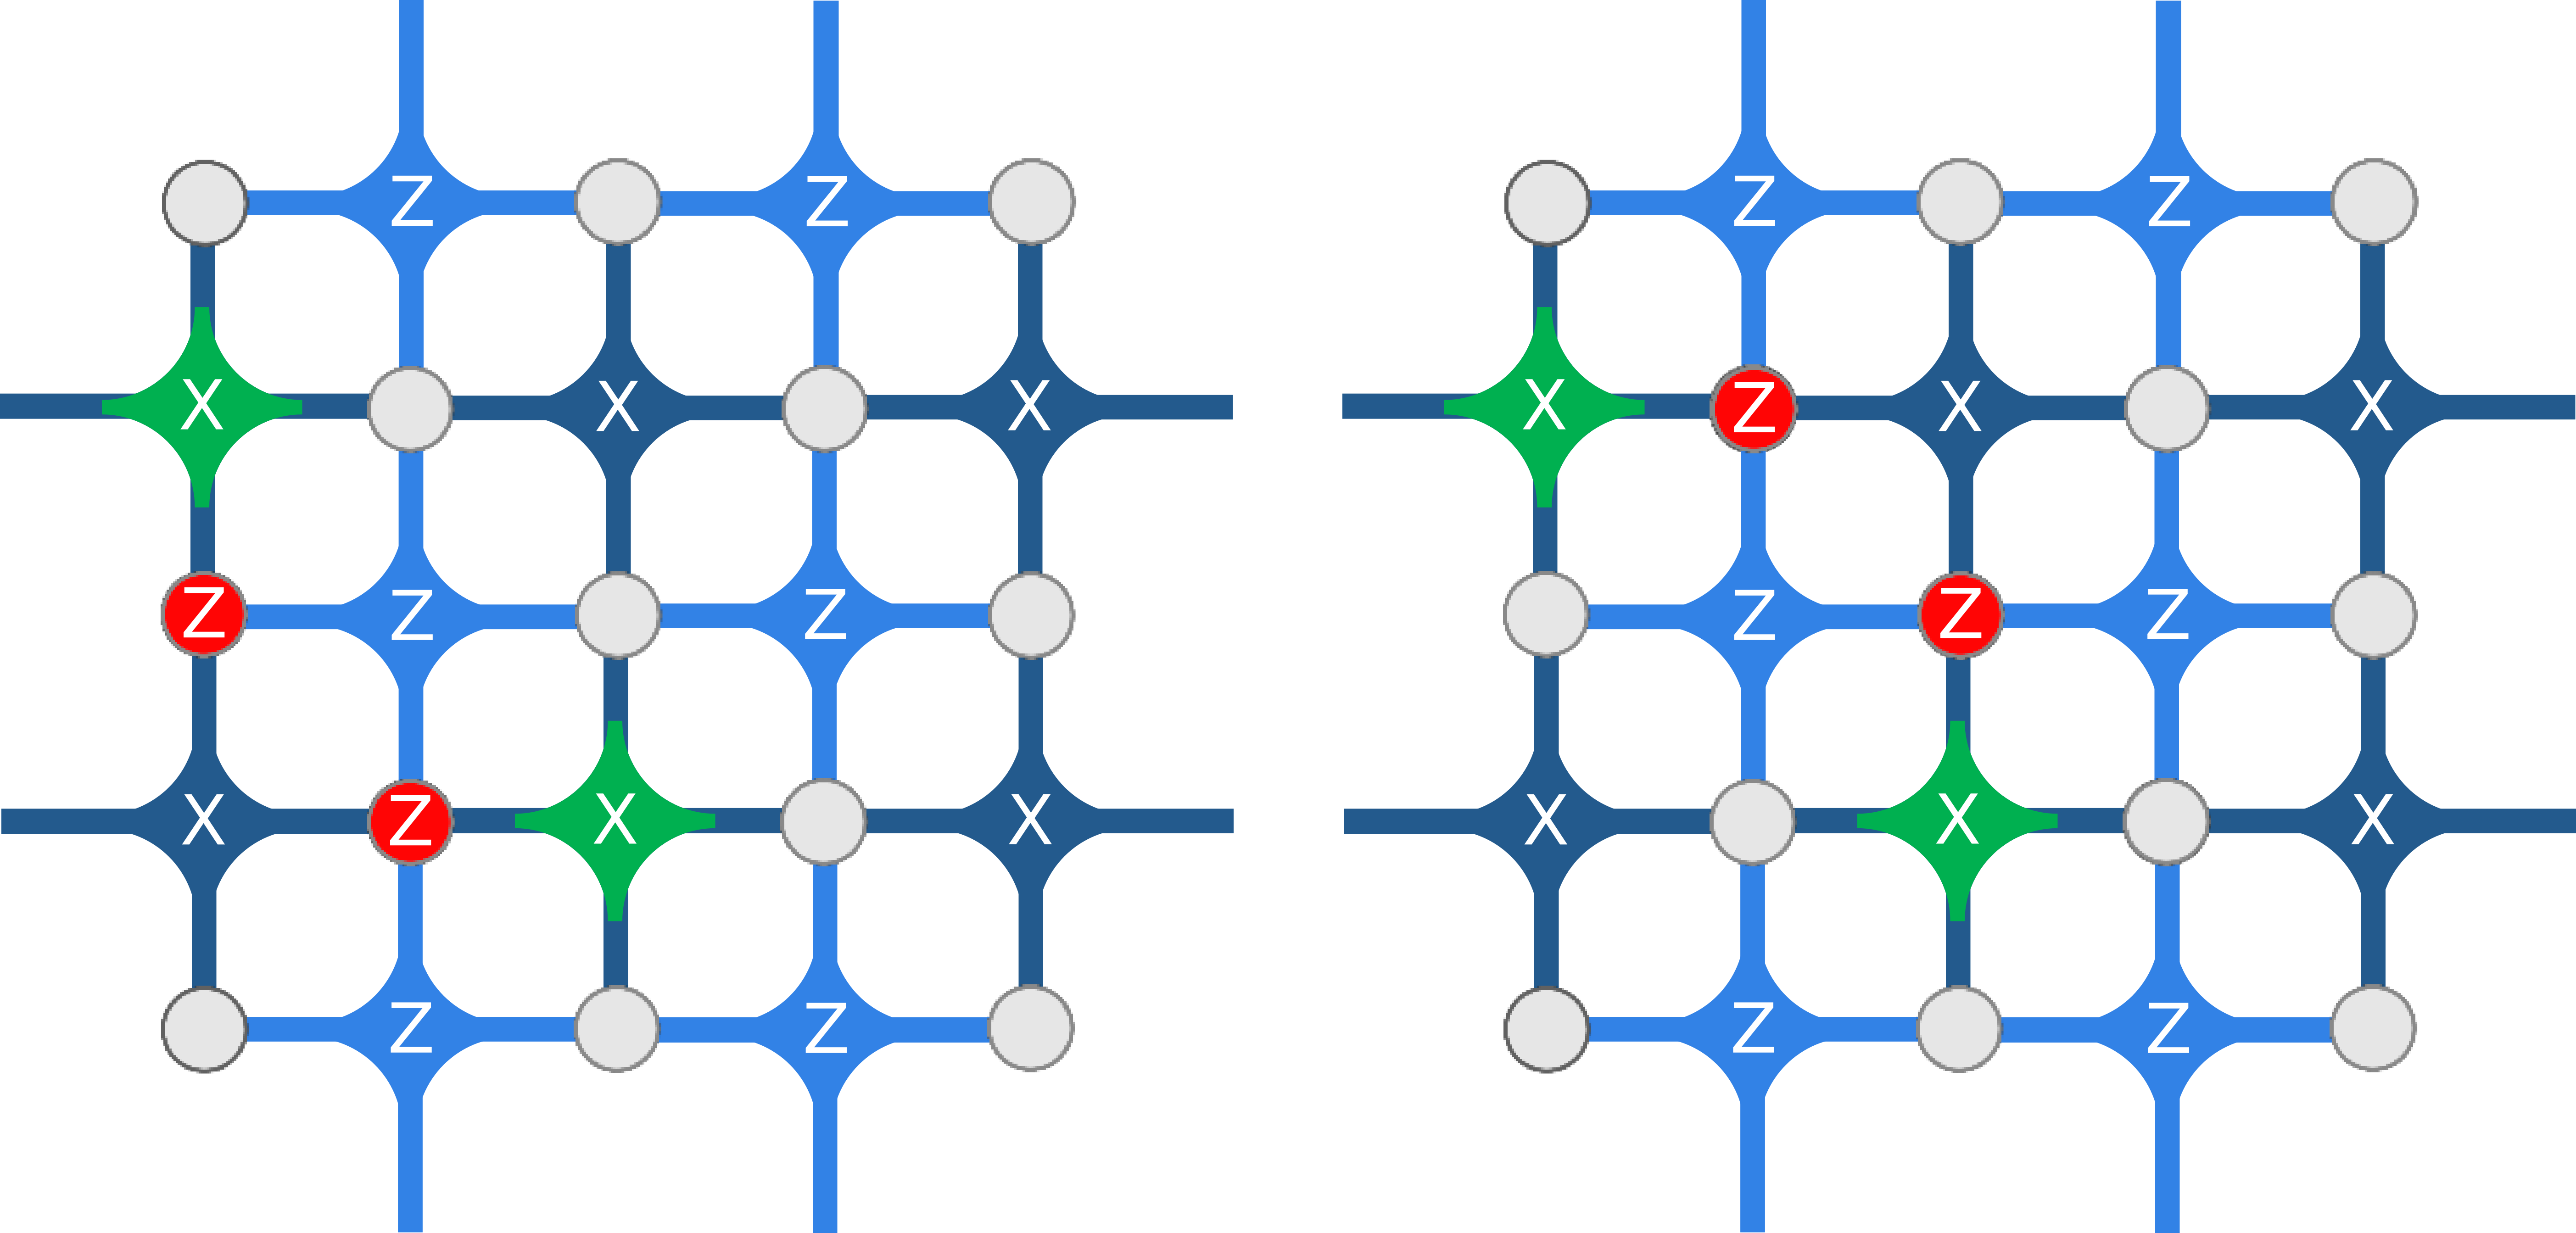
\includegraphics[height=3cm]{benign_ambiguity.png}};
      \visible<2->{
        \node at (-1.65, -3.5) {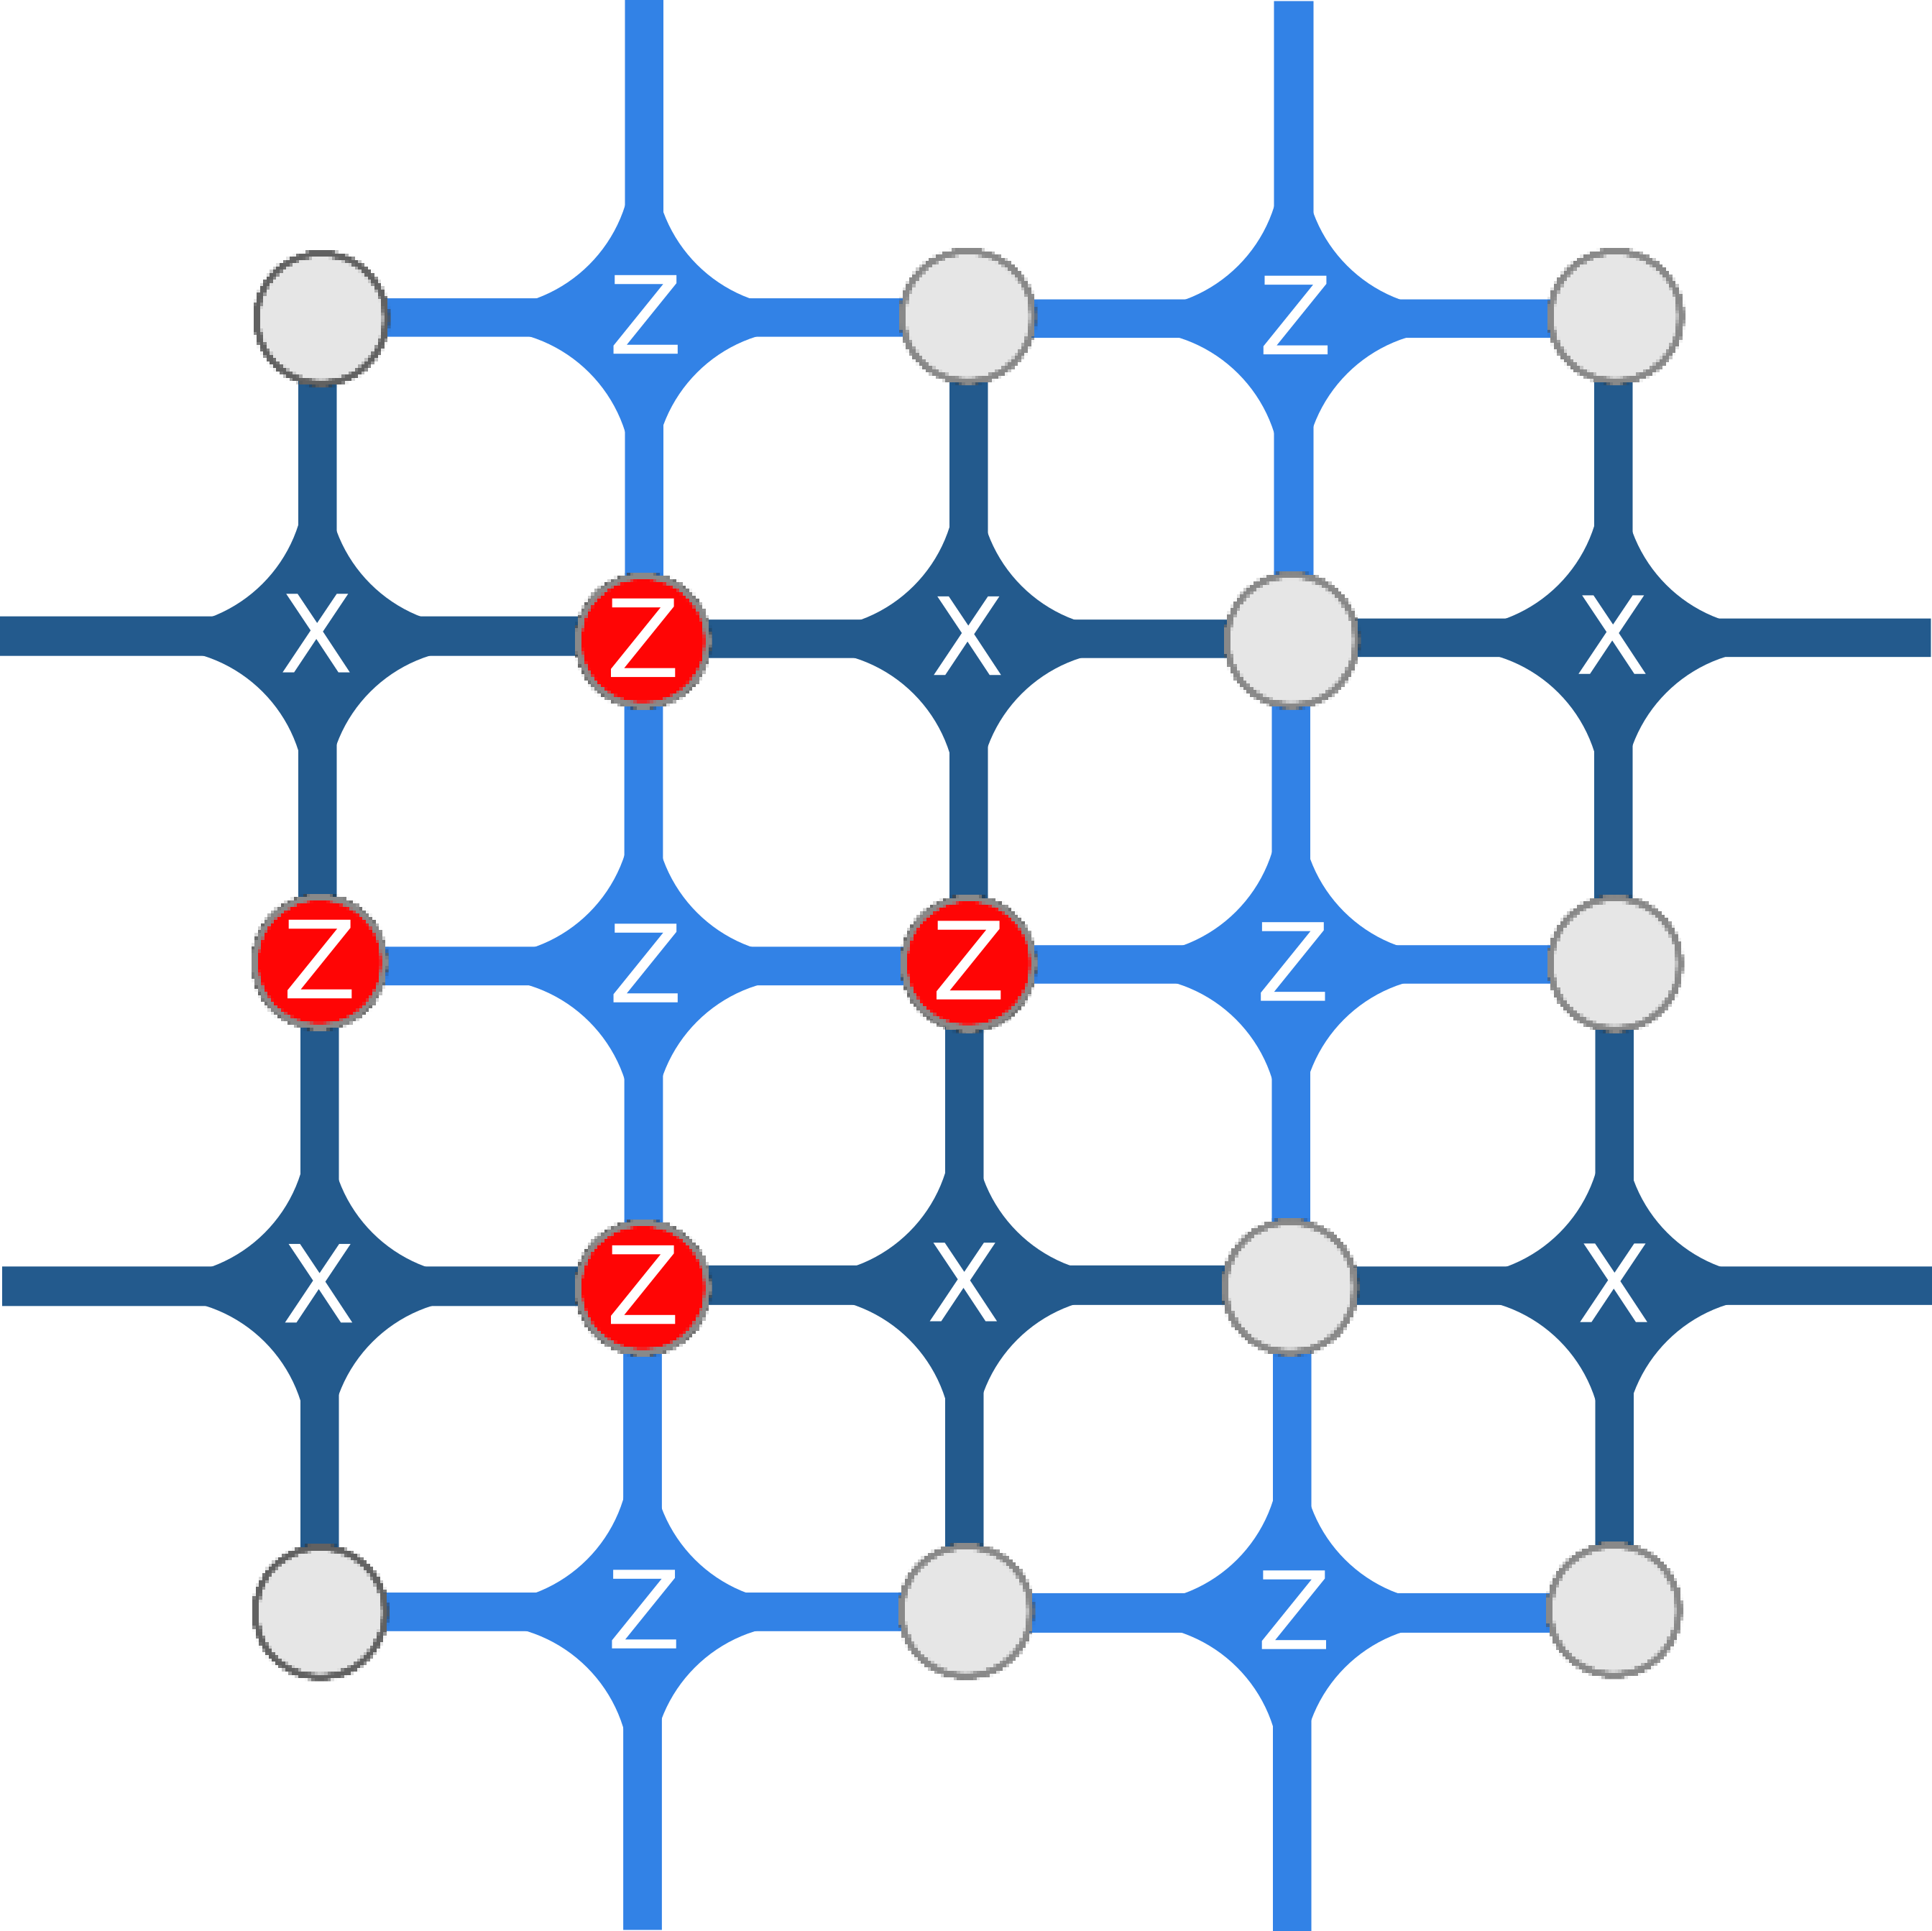
\includegraphics[height=3cm]{benign_ambiguity_loop.png}};
      }
      \visible<3->{
        \node at (1.65, -3.5) {$Error=\prod_i\sigma^z_i=Z$};
      }
    \end{tikzpicture}
  \end{center}
\end{frame}

% Real ambiguity (involving edges)
\begin{frame}{Real ambiguity}
  \begin{center}
    \begin{tikzpicture}
      \node at (0, 0) {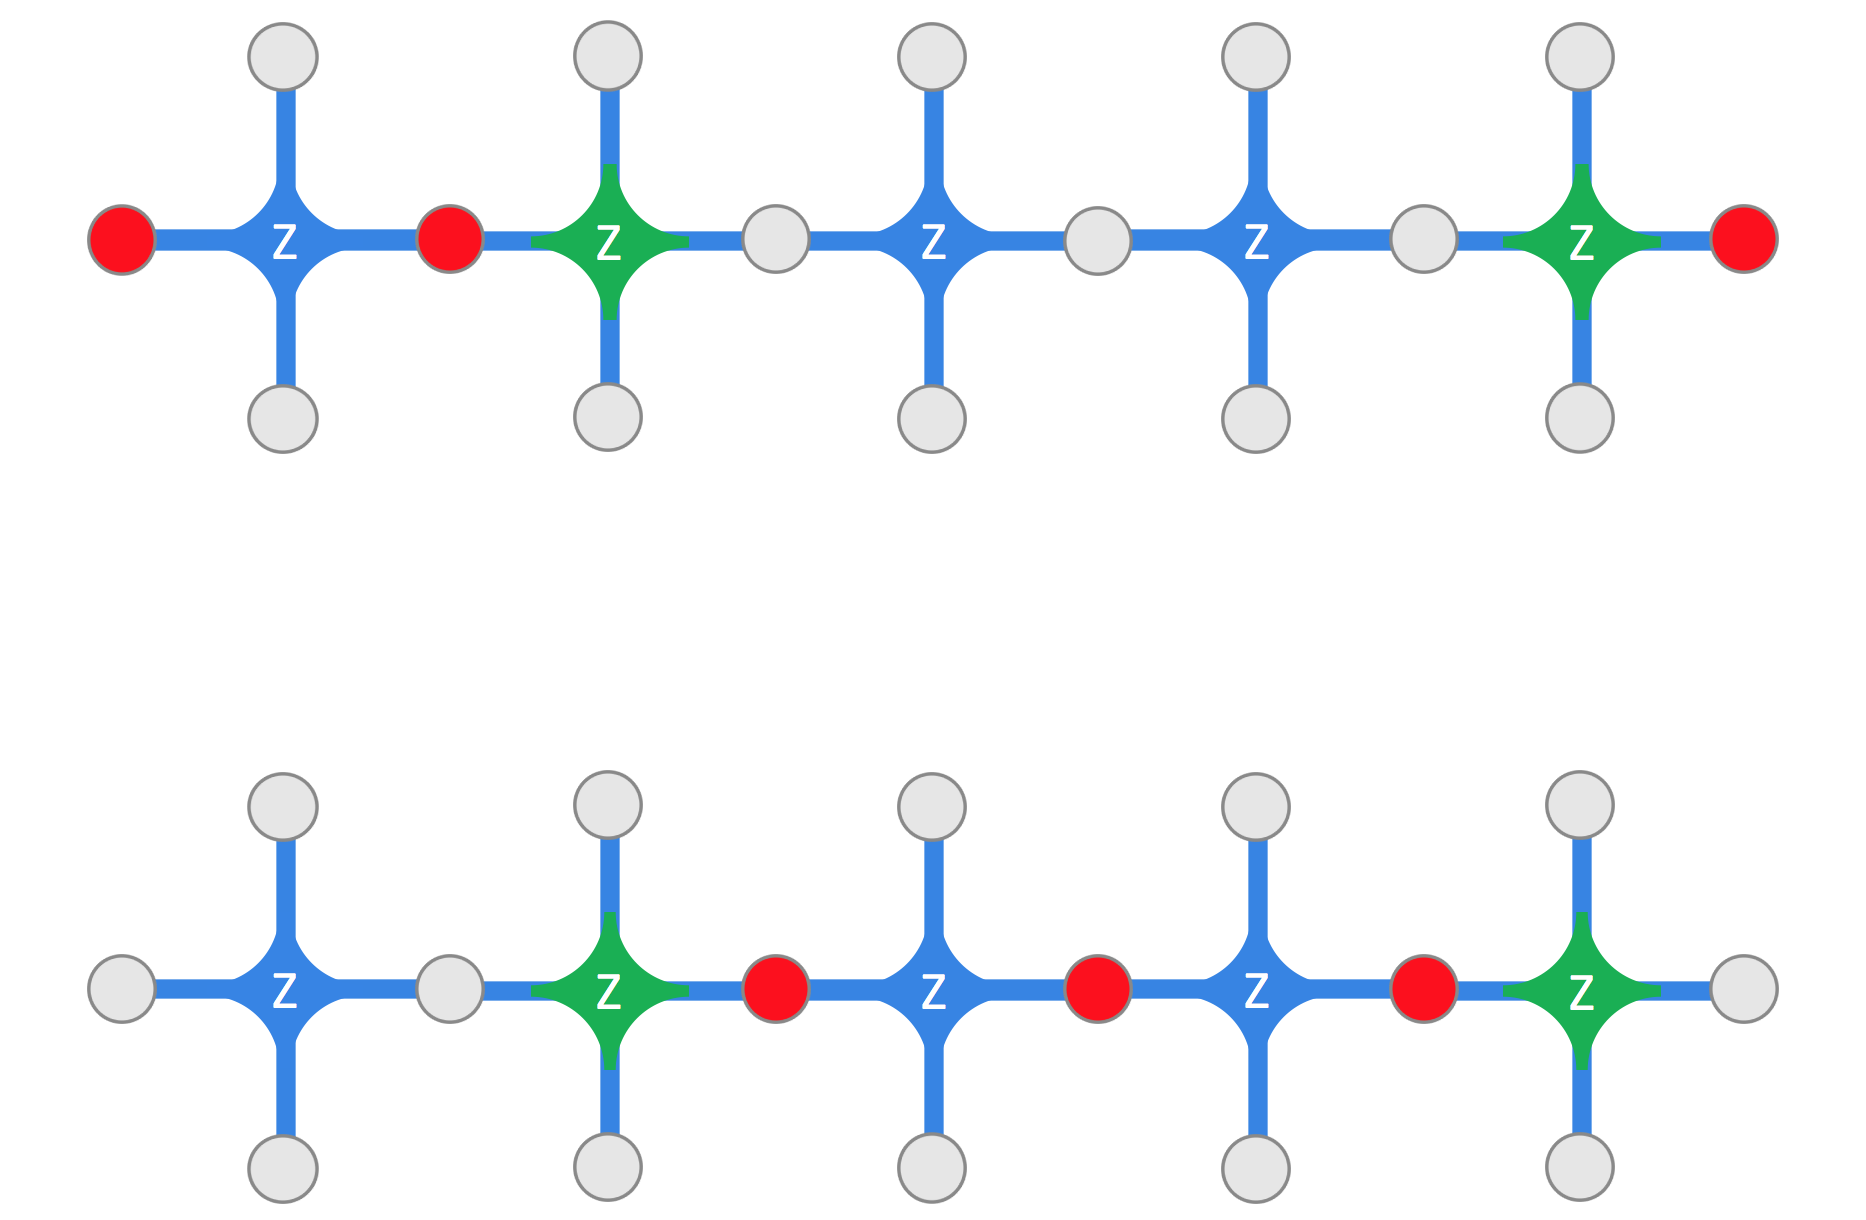
\includegraphics[height=4cm]{../2020-04-19_jc/error_degenerate.png}};
    \end{tikzpicture}
  \end{center}
\end{frame}

% Code distance
% i.e. system size

% Larger code distance
% * More redundancy
% * Less logical error (assuming independent/local single physical qubit error)
% * More processing power required
\begin{frame}{Code distance}
  \begin{center}
    \textbf{Minimal number of qubits required to form a logical error.}\\
    \visible<2->{
      i.e. system size.
    }
    \vspace{0.5cm}
    \visible<3->{
      \begin{columns}
        \column{8cm}
        \begin{block}{Larger code distance}
          \begin{itemize}
          \item<4-> More redundancy
          \item<5-> Less logical error {\small (assuming independent/local single physical qubit error)}
          \item<6-> More processing power required
          \end{itemize}
        \end{block}
      \end{columns}
    }
  \end{center}
\end{frame}

% Scaling issue
\begin{frame}{Scaling}
  \begin{center}
    \only<1>{
      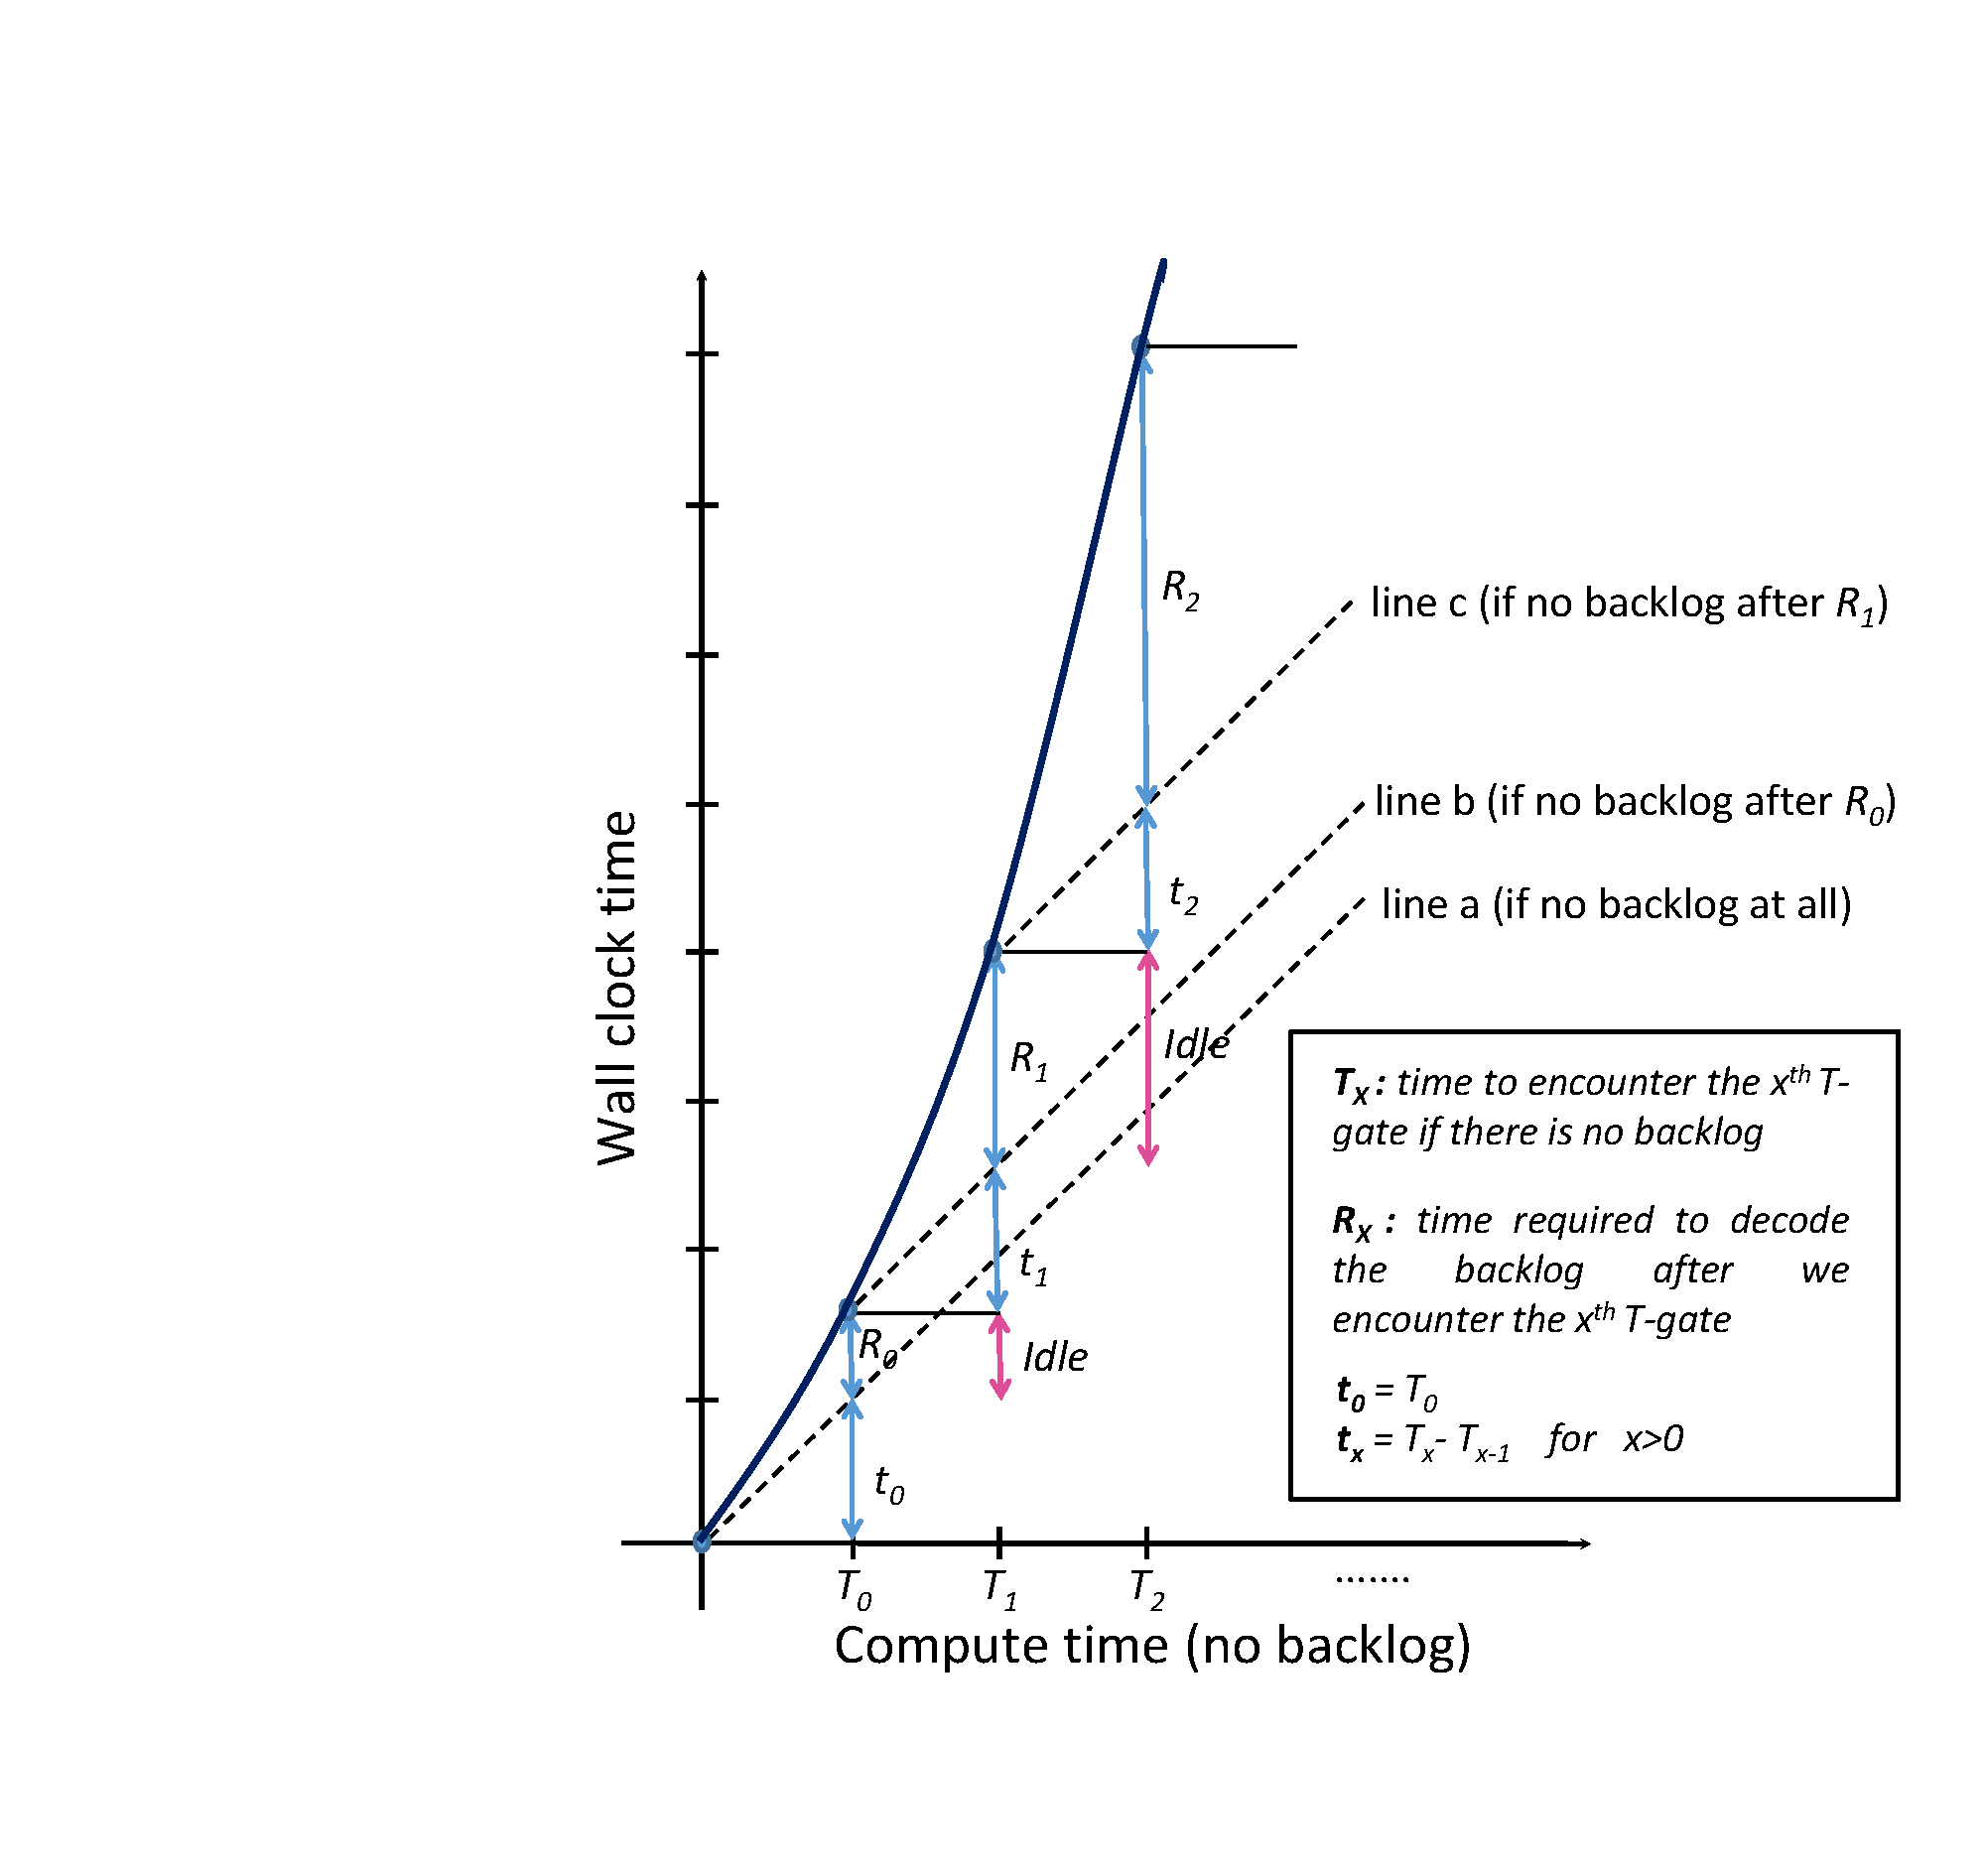
\includegraphics[height=6cm]{backlog.pdf}
    }
    \only<2>{
      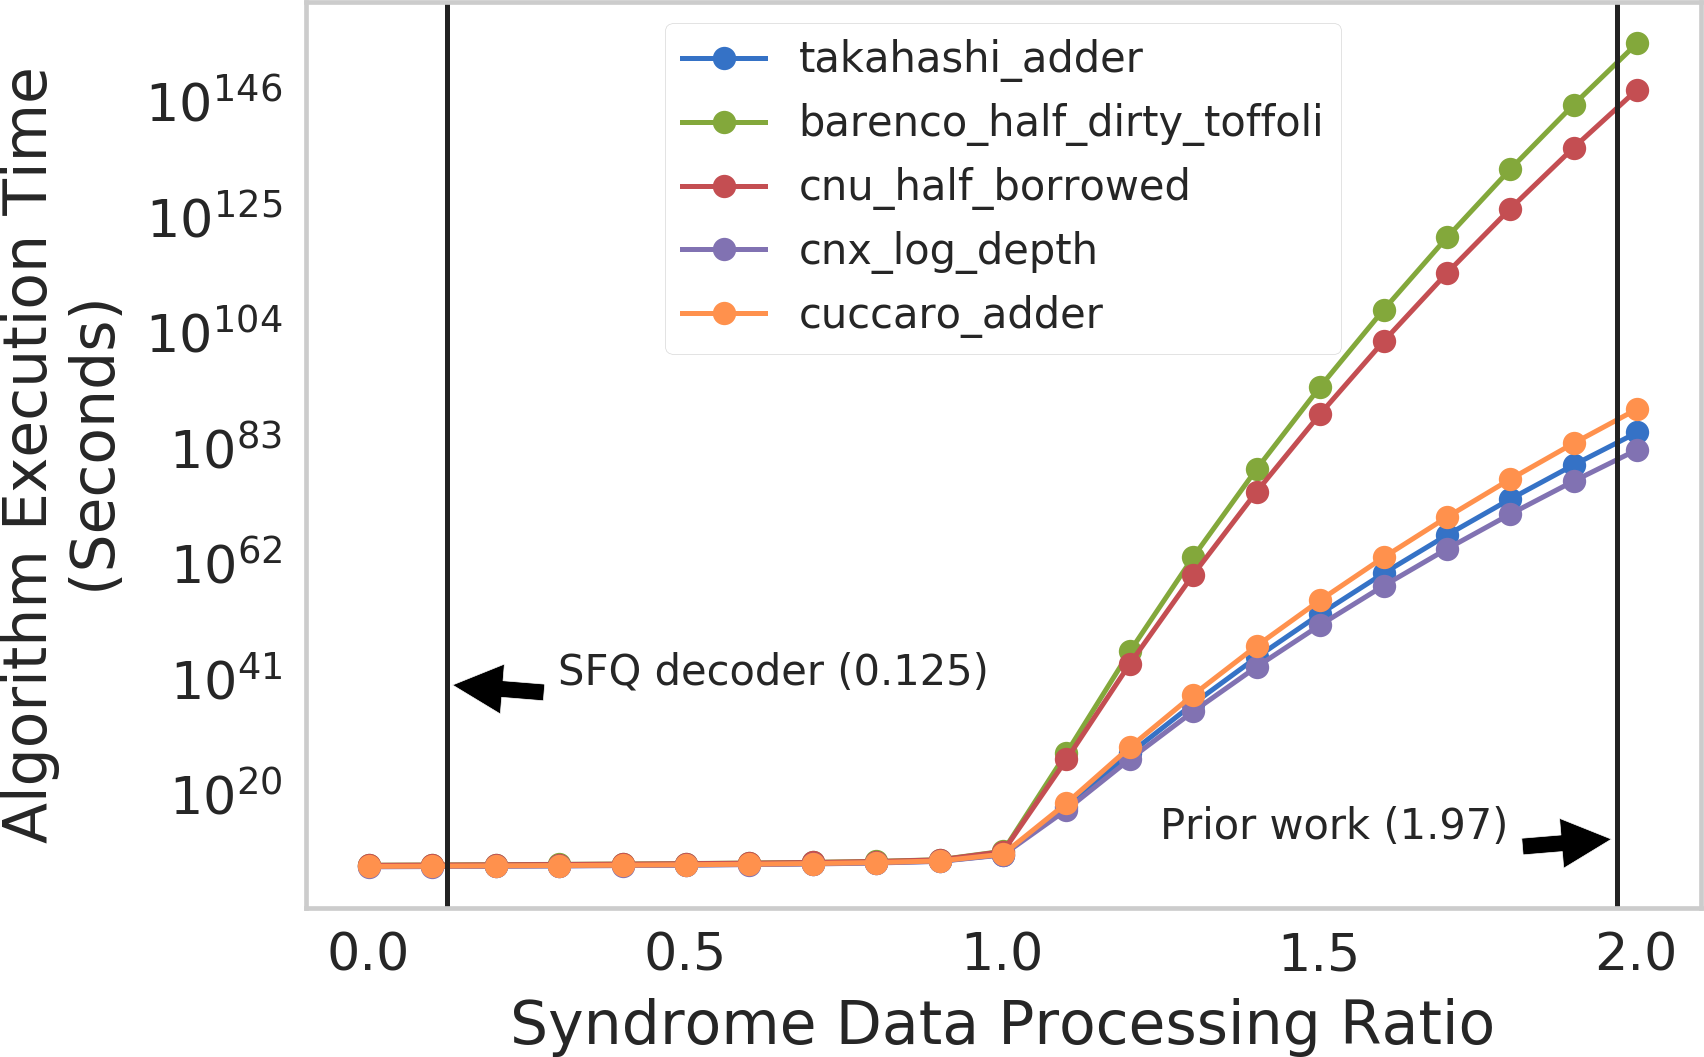
\includegraphics[height=6cm]{../2020-04-19_jc/new_scaling_plot1.png}
    }
  \end{center}
\end{frame}

% Algorithm
% Improvements
\begin{frame}{Algorithm}
  \begin{center}
    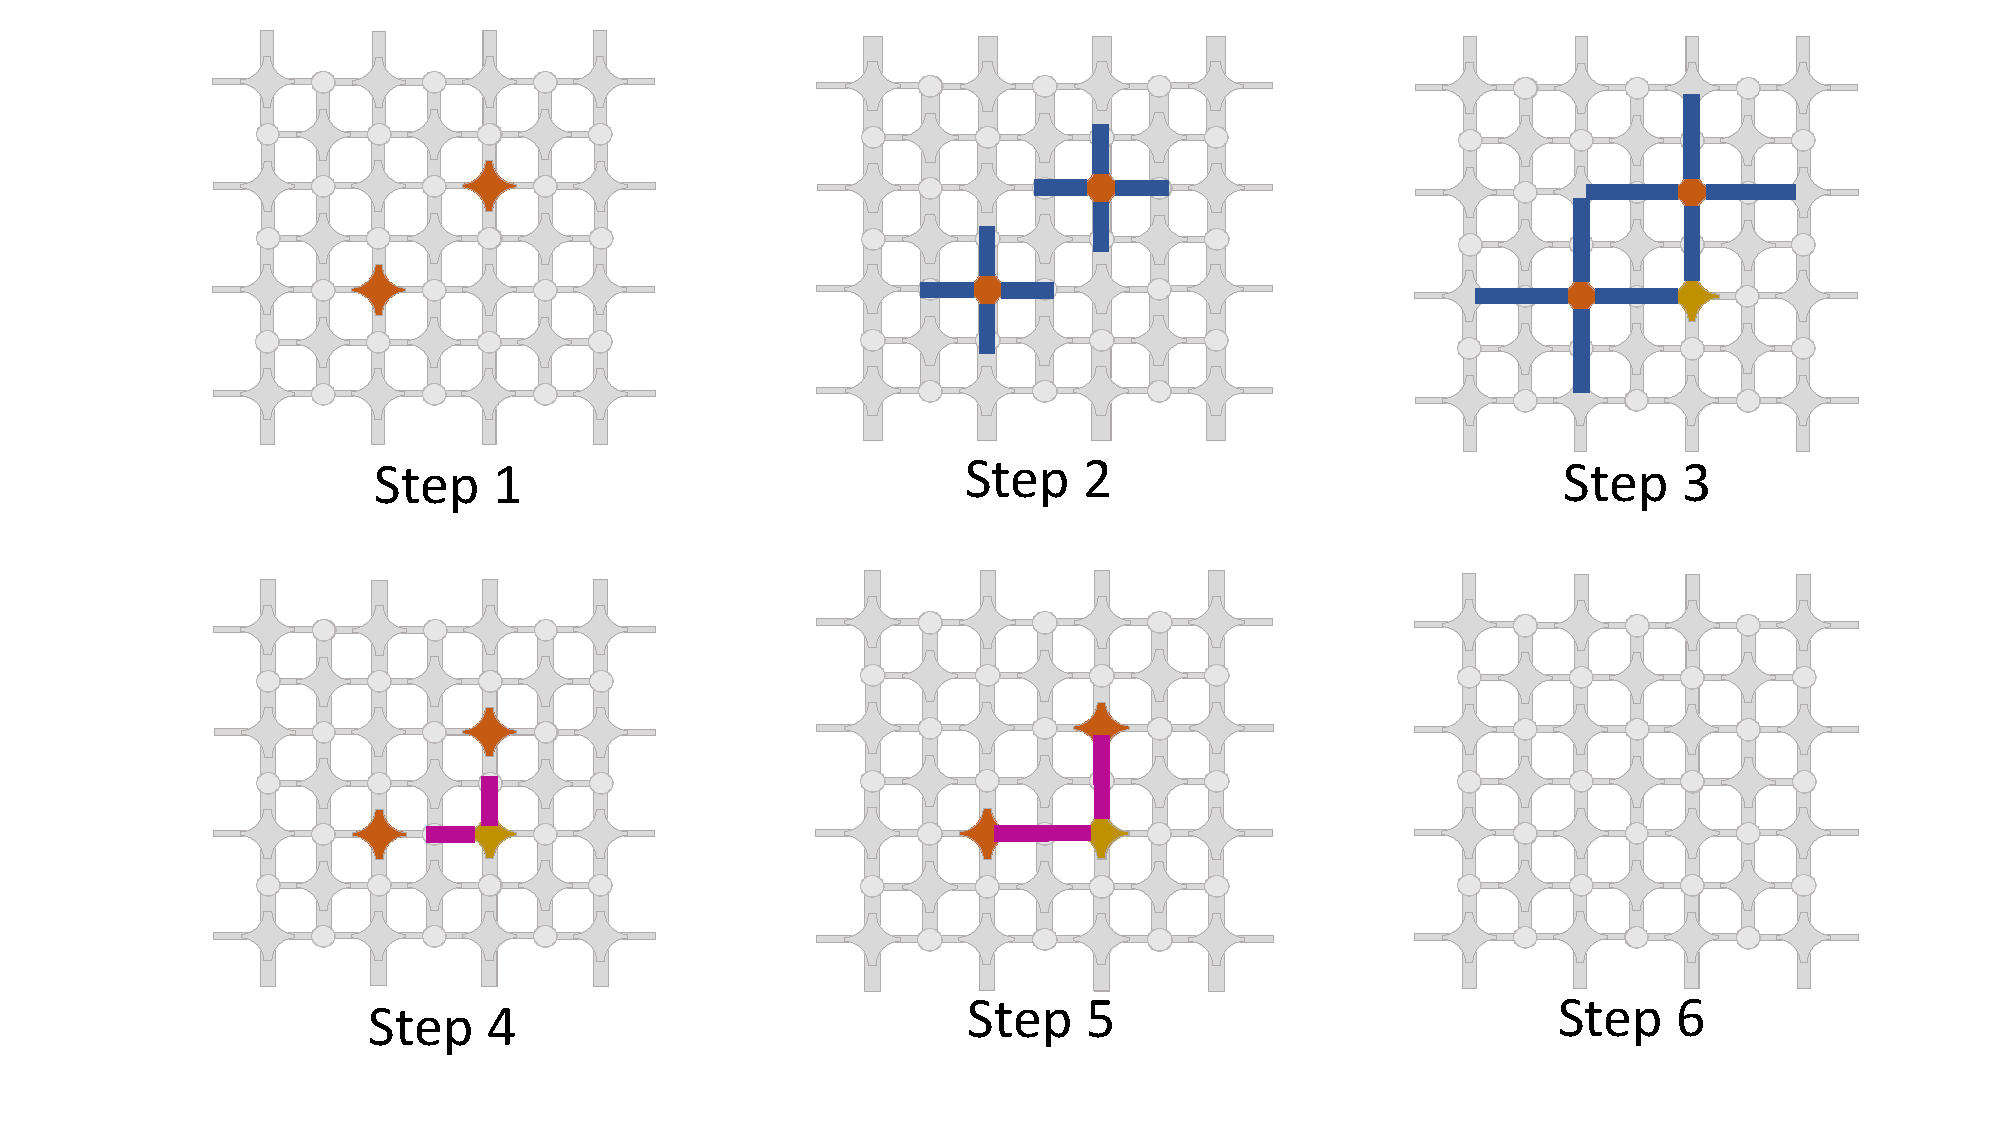
\includegraphics[width=7.5cm]{algorithm.pdf}\\
    \vspace{0.4cm}
    \visible<2->{
      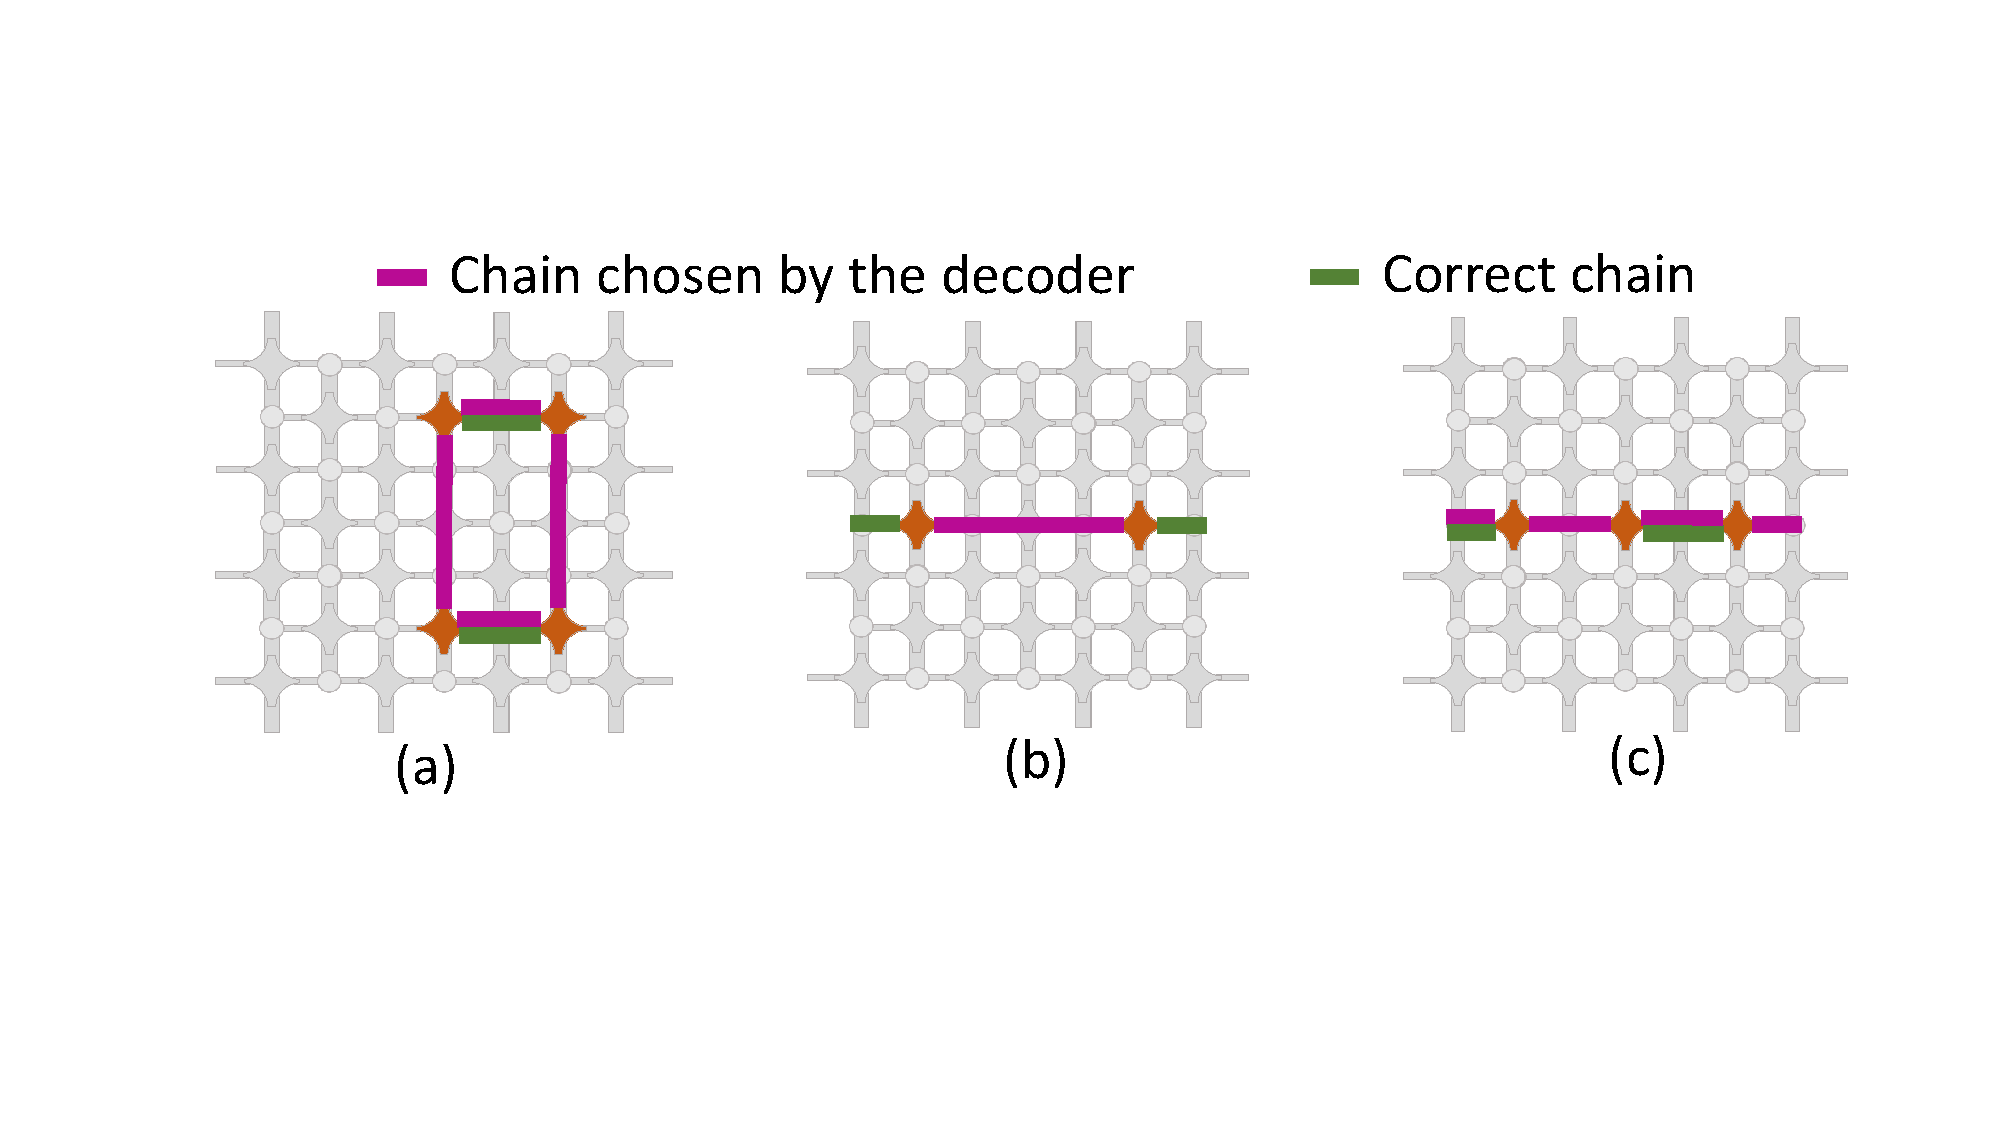
\includegraphics[width=7.5cm]{incremental-design.pdf}
    }
  \end{center}
\end{frame}

% Implementation
% Performance
\begin{frame}{Implementation and performance}
  \begin{center}
    \only<-5>{
      \begin{columns}
        \column{4.5cm}
        \begin{itemize}
        \item<1-> Hardware decoding
        \item<2-> Low power
        \item<3-> High speed
        \end{itemize}
        \column{7.3cm}
        \rowcolors{2}{gray!15}{white}
        \visible<4->{
          \begin{tabular}{rrr}
            Code Distance&Max (ns)&Average (ns)\\\hline
            3&3.74&0.28\\
            5&9.28&0.72\\
            7&14.2&2.00\\
            9&19.2&3.81
          \end{tabular}
        }
        \vspace{0.4cm}
        \visible<5->{
          \begin{center}
            \textbf{Power concumption}\\
            3.78 mW for code distance 9.
          \end{center}
        }
      \end{columns}
    }
    \only<6->{
      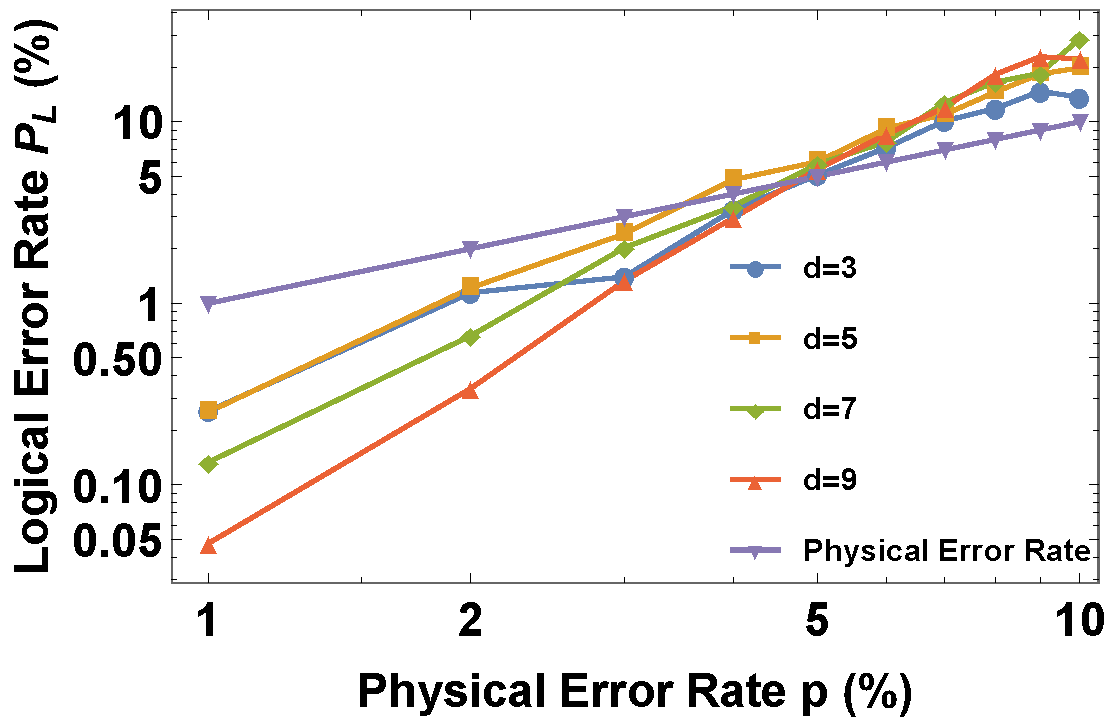
\includegraphics[width=10cm]{accuracy_threshold_dephasing_percentage.pdf}
    }
  \end{center}
\end{frame}

\end{document}
